% A small paper laid out the tex-hygiene way. Each section lives in
% sections/<slug>.tex, each result lives with its proof in theory/<slug>.tex,
% and each TikZ figure lives in tikz/<slug>.tex. In all of them, each sentence
% is on its own line. This file only says where they go. Build it with
% `latexmk -pdf main.tex`, or with three pdflatex passes.
\documentclass{article}

\usepackage{amsmath, amssymb, amsthm}
\usepackage{thmtools}
\usepackage[colorlinks=true, linkcolor=blue, citecolor=blue]{hyperref}
\usepackage{cleveref}

\usepackage{tikz}
\usetikzlibrary{arrows.meta}  % every library that a tikz/ figure needs

\theoremstyle{plain}
\newtheorem{theorem}{Theorem}
\newtheorem{proposition}{Proposition}
\newtheorem{lemma}{Lemma}
\newtheorem{corollary}{Corollary}

% After the theorem declarations, and after hyperref and cleveref.
\usepackage{deferproofs}

\newcommand{\E}{\mathbb{E}}
\newcommand{\Var}{\operatorname{Var}}
\newcommand{\Prob}{\mathbb{P}}

\begin{document}

% Each section file starts with its own heading. A section moves with its
% \input line.
\section{Setup}
\label{sec:setup}

Let $X_1, \dots, X_n$ be independent draws from a distribution with mean $\mu$ and finite variance $\sigma^2$, and let $\bar X_n = n^{-1} \sum_{i=1}^n X_i$ be their sample mean.

% An \input path starts from the folder of main.tex, also in this file.
\begin{textAtEnd}
\subsection{Proof of \autoref{thm:mean-consistency}}
\label{pf:mean-consistency}
\end{textAtEnd}
\begin{propositionE}[Consistency of the sample mean][text link={The proof is in \autoref{pf:mean-consistency}.}]
\label{thm:mean-consistency}
For every $\epsilon > 0$, the probability that the sample mean $\bar X_n$
differs from the mean $\mu$ by at least $\epsilon$ goes to zero:
\[
  \Prob\{|\bar X_n - \mu| \ge \epsilon\} \to 0
  \quad \text{as } n \to \infty.
\]
\end{propositionE}

\begin{proofE}
The draws are independent with common mean $\mu$ and common variance
$\sigma^2$, so the sample mean has mean $\E \bar X_n = \mu$ and variance
$\Var(\bar X_n) = \sigma^2 / n$. \autoref{lem:chebyshev}, applied with
$Y = \bar X_n$ and $t = \epsilon$, gives
\[
  \Prob\{|\bar X_n - \mu| \ge \epsilon\} \le \frac{\sigma^2}{n \epsilon^2},
\]
and the right side goes to zero as $n \to \infty$.
\end{proofE}

The pointer to the proof runs into this paragraph.
\Cref{fig:mean-tails} shows the probability that the proposition bounds.

% fig:mean-tails -----------------------------------------------------------
% Hand-drawn; no generator. The density of the sample mean \bar X_n, centred
% at the mean \mu, with the two tails outside the band \mu +- \epsilon shaded.
% The shaded mass is the probability that \autoref{thm:mean-consistency}
% sends to zero, and its proof bounds it with \autoref{lem:chebyshev}.
%
% Free parameters: \sd (the standard deviation of \bar X_n, in cm on the
% page), \eps (the half-width of the band, in cm) and \peak (the height of
% the curve at \mu, in cm). The curve, the tails and the label positions are
% derived from these three, so change them and the rest follows. Do not
% hardcode a coordinate. Keep \eps between 1 and 2 times \sd, so that the
% tails stay visible and the labels do not collide.
%
% Libraries: arrows.meta, loaded in the preamble.
% ---------------------------------------------------------------------------
\begin{figure}[ht]
  \centering
  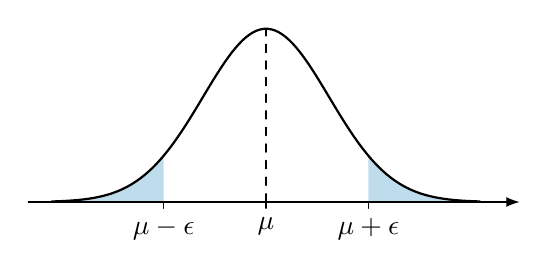
\begin{tikzpicture}[>=Latex, line cap=round, line join=round]
    \definecolor{tailblue}{HTML}{0072B2}

    % --- free parameters
    \pgfmathsetmacro{\sd}{0.8}    % standard deviation of \bar X_n, cm
    \pgfmathsetmacro{\eps}{1.3}   % half-width of the band, cm
    \pgfmathsetmacro{\peak}{2.2}  % height of the curve at \mu, cm

    % --- derived
    \pgfmathsetmacro{\reach}{3.4*\sd}  % the curve is drawn out to +- \reach

    % --- the two tails, under the curve
    \foreach \side in {-1, 1} {
      \fill[tailblue!25, domain={\side*\eps}:{\side*\reach}, samples=60]
        ({\side*\eps}, 0)
        -- plot (\x, {\peak*exp(-(\x*\x)/(2*\sd*\sd))})
        -- ({\side*\reach}, 0) -- cycle;
    }

    % --- the axis and the density
    \draw[->] ({-\reach-0.3}, 0) -- ({\reach+0.5}, 0);
    \draw[thick, domain={-\reach}:{\reach}, samples=120]
      plot (\x, {\peak*exp(-(\x*\x)/(2*\sd*\sd))});

    % --- the mean and the edges of the band, each with a tick on the axis
    \draw[dashed] (0, 0) -- (0, \peak);
    \foreach \at in {-1, 0, 1} {
      \draw ({\at*\eps}, 0) -- ({\at*\eps}, -0.08);
    }
    \node[below] at (0, -0.08) {$\mu$};
    \node[below] at ({-\eps}, -0.08) {$\mu - \epsilon$};
    \node[below] at ({\eps}, -0.08) {$\mu + \epsilon$};
  \end{tikzpicture}
  \caption{The density of the sample mean $\bar X_n$.
    The shaded tails are the probability that $\bar X_n$ differs from $\mu$ by at least $\epsilon$.}
  \label{fig:mean-tails}
\end{figure}



\appendix
\section{Proofs}
\label{sec:proofs}

\subsection{A supporting lemma}

% A result that is stated and proved in the appendix uses the plain
% environments, and its file is input where it belongs.
\begin{lemma}[Chebyshev's inequality]
\label{lem:chebyshev}
Let $Y$ be a random variable with finite variance.
For every $t > 0$,
\[
  \Prob\{|Y - \E Y| \ge t\} \le \frac{\Var(Y)}{t^2}.
\]
\end{lemma}

\begin{proof}
The event $|Y - \E Y| \ge t$ is the event $(Y - \E Y)^2 \ge t^2$.
Markov's inequality, applied to the nonnegative random variable $(Y - \E Y)^2$ at the level $t^2$, bounds its probability by $\E[(Y - \E Y)^2] / t^2$, which is $\Var(Y) / t^2$.
\end{proof}


% Every deferred proof, in the order its statement appears in the body. Each
% one brings its own subsection heading from the textAtEnd block in its file.
\printProofs


\end{document}
